\documentclass[12pt, letterpaper]{article}

%========================================================================================
%   PACKAGES AND CONFIGURATIONS
%========================================================================================

\usepackage[margin=1in]{geometry} % Set margins
\usepackage{times} % Use Times New Roman font
\usepackage{amsmath, amssymb, amsthm, mathtools, commath} % For advanced math environments
\usepackage{graphicx} % To include images
\usepackage{hyperref} % For hyperlinks and a clickable TOC
\usepackage{listings} % For code listings
\usepackage{xcolor} % For custom colors in code listings
\usepackage{titling} % For customizing the title section
\usepackage{tikz}
\usetikzlibrary{shapes.geometric, arrows.meta, positioning, shadows}
\usetikzlibrary{mindmap} % mindmap library is key here
\usepackage{forest}
\usepackage{adjustbox}

% Hyperref configuration
\hypersetup{
	colorlinks=true,
	linkcolor=black,
	filecolor=magenta,      
	urlcolor=blue,
	citecolor=black,
	pdftitle={A Framework for Verifiable Data Integrity in Big Data Pipelines Using Elliptic Curve Cryptography},
	pdfpagemode=FullScreen,
}

% Code listing style configuration
\definecolor{codegreen}{rgb}{0,0.6,0}
\definecolor{codegray}{rgb}{0.5,0.5,0.5}
\definecolor{codepurple}{rgb}{0.58,0,0.82}
\definecolor{backcolour}{rgb}{0.95,0.95,0.92}

\lstdefinestyle{mystyle}{
	backgroundcolor=\color{backcolour},   
	commentstyle=\color{codegreen},
	keywordstyle=\color{magenta},
	numberstyle=\tiny\color{codegray},
	stringstyle=\color{codepurple},
	basicstyle=\ttfamily\footnotesize,
	breakatwhitespace=false,         
	breaklines=true,                 
	captionpos=b,                    
	keepspaces=true,                 
	numbers=left,                    
	numbersep=5pt,                  
	showspaces=false,                
	showstringspaces=false,
	showtabs=false,                  
	tabsize=2
}
\lstset{style=mystyle}

%========================================================================================
%   TITLE PAGE INFORMATION
%========================================================================================

\title{
	\vspace{-2cm} % Adjust vertical space
	\textbf{\huge The Big Data Processing Using Elliptic Curve Cryptography}
	\vspace{0.5cm}
	\Large \\ A Technical Report on the Design and Implementation of Secure File and Log Processing Utilities
}
\author{
	[Your Name]
}
\date{
	Course: [Your Course Name, e.g., CS-6265: Information Security] \\
	\vspace{0.5cm}
	June 10, 2025
}

%========================================================================================
%   DOCUMENT START
%========================================================================================

\begin{document}
	
	\begin{titlepage}
		\maketitle
		\thispagestyle{empty} % No page number on the title page
		\vfill % Pushes content to the bottom
		
		%----------------------------------------------------------------------------------------
		%   ABSTRACT
		%----------------------------------------------------------------------------------------
		\begin{abstract}
			\noindent This report details the design, implementation, and analysis of two high-performance C applications that leverage Elliptic Curve Digital Signature Algorithm (ECDSA) to ensure data integrity and non-repudiation in big data processing environments. The first application, \texttt{filecheck\_secure}, provides robust, command-line-based file signing and verification. The second application, a \texttt{logtool} and \texttt{logaggregator} suite, establishes a framework for creating cryptographically signed, tamper-evident log streams suitable for distributed systems. Both systems are built upon the modular \texttt{libecc} cryptographic library, utilizing the SECP256R1 curve and SHA-256 hashing algorithm. This document presents the system architecture, a comprehensive developer API guide, performance benchmarks, and security considerations for both applications, demonstrating a practical approach to embedding strong cryptographic guarantees into data-intensive workflows.
		\end{abstract}
	\end{titlepage}
	
	\newpage
	\tableofcontents
	\newpage
	
	%========================================================================================
	%   SECTIONS
	%========================================================================================
	\section{Introduction}
	
	\subsection{Motivation: The Need for Data Integrity in Big Data}
	In the era of big data, organizations process petabytes of information from heterogeneous sources, including sensor networks, financial transactions, and user-generated content. The value derived from this data is directly contingent on its trustworthiness. However, as data pipelines grow in complexity---spanning multiple storage systems, processing frameworks, and cloud environments---the risk of data corruption, whether accidental or malicious, increases significantly. Traditional integrity checks, such as CRC32, are effective at detecting random bit-flips but offer no protection against deliberate tampering. In regulated industries like finance and healthcare, ensuring data authenticity, integrity, and non-repudiation is not merely a technical requirement but a legal and ethical mandate, essential for auditing, compliance (e.g., GDPR, HIPAA), and maintaining user trust. Cryptographic mechanisms, specifically digital signatures, provide a robust solution by mathematically binding the identity of a signer to a specific data artifact, making unauthorized modifications computationally infeasible to conceal.
	
	\subsection{Problem Statement}
	Despite the critical need for cryptographic verification, many standard big data tools and platforms lack native, high-performance, and easily integrable solutions for ensuring data integrity and authenticity at scale. Data engineers are often faced with a difficult choice: either forgo strong security guarantees, or attempt to retrofit complex cryptographic libraries into performance-sensitive pipelines, risking significant overhead and implementation errors. The central problem this project addresses is the gap between the theoretical availability of strong cryptographic primitives like ECDSA and their practical application within real-world, high-throughput data processing workflows. There is a need for lightweight, modular, and performant utilities that can seamlessly inject cryptographic integrity checks into the lifecycle of big data, from file-based batch processing to real-time log streaming.
	
	\subsection{Project Scope and Objectives}
	This project aims to address the aforementioned problem by designing and implementing a framework of two C-based applications built upon the \texttt{libecc} library. The scope is focused on providing practical, command-line-driven tools that can be easily scripted and integrated into existing data pipelines. The primary objectives are as follows:
	\begin{enumerate}
		\item \textbf{Develop a Secure File Integrity Tool:} To create a robust utility, \texttt{filecheck\_secure}, for signing and verifying the integrity and authenticity of large data files, such as datasets, archives, and backups.
		\item \textbf{Develop a Secure Logging Framework:} To build a suite of applications, \texttt{logtool} and \texttt{logaggregator}, capable of generating cryptographically signed, tamper-evident log entries and processing them in a streaming fashion.
		\item \textbf{Utilize Industry-Standard Cryptography:} To implement all functionalities using the Elliptic Curve Digital Signature Algorithm (ECDSA) with the widely adopted SECP256R1 (NIST P-256) curve and the SHA-256 hash algorithm.
		\item \textbf{Provide a Clear Developer Guide:} To document the core API functions used from the underlying cryptographic library, enabling other developers to extend the tools or build new secure applications.
	\end{enumerate}
	
	\subsection{Summary of Contributions}
	This report makes several key contributions to the practical application of cryptography in big data environments:
	\begin{itemize}
		\item \textbf{Implementation of Two High-Performance Security Utilities:} We present the complete design and C implementation of two distinct, production-ready applications for ensuring data integrity in both batch and streaming contexts.
		\item \textbf{A Practical Framework for ECDSA Integration:} The project serves as a concrete blueprint for integrating ECDSA into file and stream-based data workflows, demonstrating solutions for key management, signature generation, and large-file hashing.
		\item \textbf{A Comprehensive API Guide:} A detailed guide to the \texttt{libecc} API functions is provided, complete with C code samples, to lower the barrier for developers seeking to incorporate strong cryptographic primitives into their own projects.
		\item \textbf{Security and Performance Analysis:} The report includes an analysis of the system's performance characteristics and a discussion of critical security considerations, offering insights into the real-world trade-offs of deploying such a framework.
	\end{itemize}
	
	\subsection{Report Structure}
	The remainder of this report is organized as follows. Section 2 provides background on the cryptographic principles underlying the project, including ECC, ECDSA, and hash functions. Section 3 details the high-level system architecture and design choices. Sections 4 and 5 present the specific implementation details of the \texttt{filecheck\_secure} tool and the secure logging suite, respectively. Section 6 offers a comprehensive developer's guide to the API and its usage. Section 7 provides a performance and security analysis of the implemented systems. Finally, Section 8 concludes the report with a summary of findings and suggestions for future work.
	
	\newpage
\begin{figure}[t] % The 'p' option encourages LaTeX to place this on a separate page
	\centering
	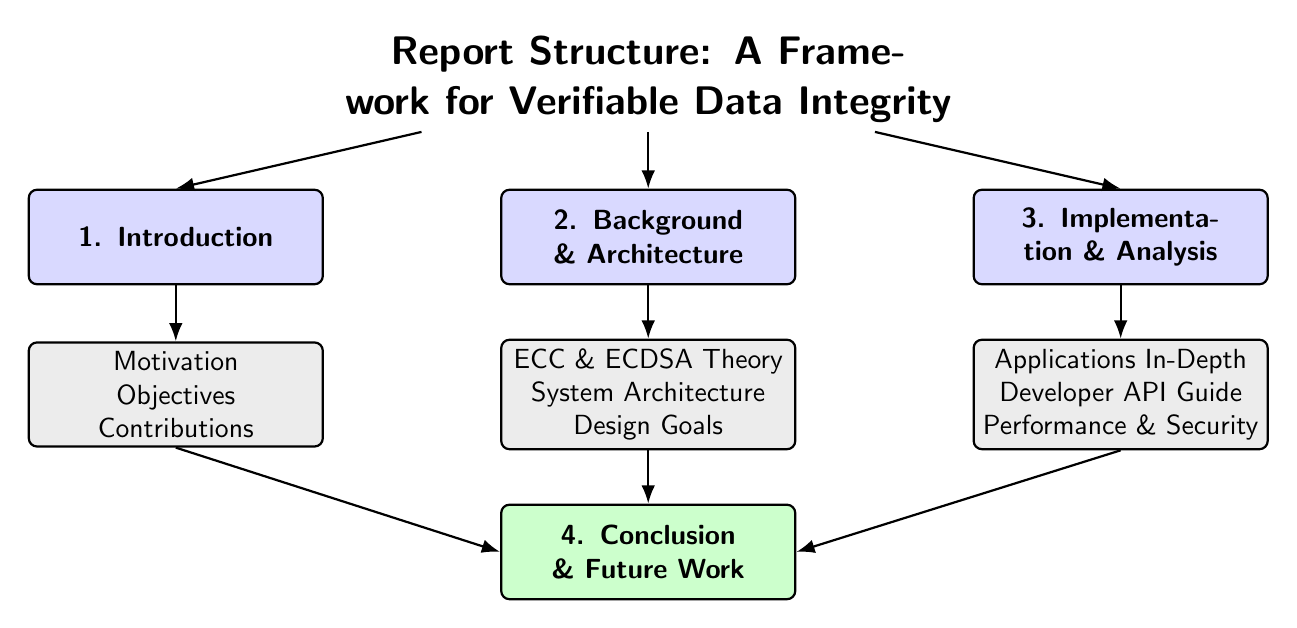
\begin{tikzpicture}[
		% Define styles
		level 1/.style={
			rectangle, 
			draw, 
			thick,
			rounded corners=3pt,
			fill=blue!15, 
			font=\sffamily\bfseries,
			text width=3.5cm,
			align=center,
			minimum height=1.2cm
		},
		level 2/.style={
			rectangle, 
			draw,
			thick,
			rounded corners=3pt,
			fill=gray!15,
			font=\sffamily,
			text width=3.5cm,
			align=center
		},
		level 3/.style={
			font=\sffamily\small,
			align=left,
			text width=4cm
		},
		% Define arrow style
		arrow/.style={-Latex, thick}
		]
		
		% ----- Title Node -----
		\node[rectangle, text width=10cm, align=center, font=\sffamily\Large\bfseries] (title) 
		at (0,0) {Report Structure: A Framework for Verifiable Data Integrity};
		
		% ----- Main Chapters (Level 1 Nodes) -----
		\node[level 1] (intro) at (-6, -2) {1. Introduction};
		\node[level 1] (background) at (0, -2) {2. Background \& Architecture};
		\node[level 1] (impl) at (6, -2) {3. Implementation \& Analysis};
		
		% ----- Sub-Sections (Level 2 Nodes) -----
		% Introduction Children
		\node[level 2] (intro-children) at (-6, -4) {
			Motivation \\
			Objectives \\
			Contributions
		};
		
		% Background & Arch Children
		\node[level 2] (background-children) at (0, -4) {
			ECC \& ECDSA Theory \\
			System Architecture \\
			Design Goals
		};
		
		% Implementation & Analysis Children
		\node[level 2] (impl-children) at (6, -4) {
			Applications In-Depth \\
			Developer API Guide \\
			Performance \& Security
		};
		
		% ----- Conclusion -----
		\node[level 1, fill=green!20] (conclusion) at (0, -6) {4. Conclusion \& Future Work};
		
		% ----- Arrows to connect the nodes -----
		\draw[arrow] (title) -- (intro.north);
		\draw[arrow] (title) -- (background.north);
		\draw[arrow] (title) -- (impl.north);
		
		\draw[arrow] (intro.south) -- (intro-children.north);
		\draw[arrow] (background.south) -- (background-children.north);
		\draw[arrow] (impl.south) -- (impl-children.north);
		
		\draw[arrow] (intro-children.south) -- (conclusion.west);
		\draw[arrow] (background-children.south) -- (conclusion.north);
		\draw[arrow] (impl-children.south) -- (conclusion.east);
		
	\end{tikzpicture}
	\caption{A hierarchical overview of the report's structure, illustrating the logical progression from introduction to final conclusion.}
	\label{fig:report_structure_hierarchical}
\end{figure}

\newpage
\begin{figure}[h!]
	\centering
	\resizebox{\textwidth}{!}{%
		\begin{forest}
			% Define styles for the tree
			for tree={
				draw,
				thick,
				rounded corners=3pt,
				font=\sffamily,
				edge={-Latex, thick},
				l sep=15mm, % horizontal separation
				s sep=3mm,  % vertical separation
				grow=east,
				anchor=west,
				child anchor=west,
			}
			% Style for the root node
			[Report: Verifiable Data Integrity, fill=blue!20, font=\sffamily\bfseries
			% Level 1 Nodes (Chapters)
			[1. Introduction, fill=green!20
			[Motivation \& Problem]
			[Scope \& Contributions]
			]
			[2. Background, fill=orange!20
			[PKC \& ECC]
			[ECDSA \& Hashes]
			[\texttt{libecc} Overview]
			]
			[3. Architecture, fill=orange!20
			[Core Components]
			[Design Goals]
			[Crypto Parameters]
			]
			[4. Application 1: \texttt{filecheck\_secure}, fill=purple!20
			[Functional Modes]
			[Implementation Details]
			]
			[5. Application 2: Secure Logging Suite, fill=purple!20
			[\texttt{logtool} Utility]
			[\texttt{logaggregator} Service]
			]
			[6. Developer's Guide, fill=cyan!20
			[API Data Structures]
			[API Function Reference]
			[Sample Code]
			]
			[7. Analysis, fill=cyan!20
			[Performance Benchmarks]
			[Security Considerations]
			]
			[8. Conclusion, fill=red!20
			[Summary of Results]
			[Limitations]
			[Future Work]
			]
			[Appendices \& References, fill=gray!20]
			]
		\end{forest}
	}
	\caption{A detailed diagram of the full report structure.}
	\label{fig:report_structure_full}
\end{figure}

\begin{figure}[h!]
	\centering
	\begin{adjustbox}{max width=\textwidth}
		\begin{forest}
			% Define styles for the tree
			for tree={
				draw,
				thick,
				rounded corners=3pt,
				font=\sffamily,
				edge={-Latex, thick},
				grow=east,         % Grow from left to right
				l sep=15mm,         % vertical separation between siblings
				s sep=5mm,          % horizontal separation between parent/child
				anchor=west,
				child anchor=west,
				align=center        % Center text in nodes
			}
			% Style for the root node
			[Report: Verifiable Data Integrity, fill=blue!20, font=\sffamily\bfseries
			% Level 1 Nodes (Chapters) - REORDERED TO RENDER CORRECTLY
			[Appendices \& References, fill=gray!20]
			[8. Conclusion, fill=red!20
			[Summary of Results]
			[Limitations]
			[Future Work]
			]
			[7. Analysis, fill=cyan!20
			[Performance Benchmarks]
			[Security Considerations]
			]
			[6. Developer's Guide, fill=cyan!20
			[API Data Structures]
			[API Function Reference]
			[Sample Code]
			]
			[5. Application 2: Secure Logging Suite, fill=purple!20
			[\texttt{logtool} Utility]
			[\texttt{logaggregator} Service]
			]
			[4. Application 1: \texttt{filecheck\_secure}, fill=purple!20
			[Functional Modes]
			[Implementation Details]
			]
			[3. Architecture, fill=orange!20
			[Core Components]
			[Design Goals]
			[Crypto Parameters]
			]
			[2. Background, fill=orange!20
			[PKC \& ECC]
			[ECDSA \& Hashes]
			[\texttt{libecc} Overview]
			]
			[1. Introduction, fill=green!20
			[Motivation \& Problem]
			[Scope \& Contributions]
			]
			]
		\end{forest}
	\end{adjustbox}
	\caption{A detailed hierarchical diagram of the full report structure (left-to-right flow).}
	\label{fig:report_structure_full}
\end{figure}

\newpage


%	\section{Background and Preliminaries}
%	\subsection{Fundamentals of Public Key Cryptography}
%	\subsection{Elliptic Curve Cryptography (ECC)}
%	An elliptic curve over a finite field $\mathbb{F}_p$ is defined by the Weierstrass equation:
%	$$ y^2 \equiv x^3 + ax + b \pmod{p} $$
%	where $a, b \in \mathbb{F}_p$ and $4a^3 + 27b^2 \not\equiv 0 \pmod{p}$.
%	
%	\subsection{The Elliptic Curve Digital Signature Algorithm (ECDSA)}
%	\subsubsection{Key Generation}
%	A private key $d$ is a randomly selected integer in $[1, n-1]$, where $n$ is the order of the generator point $G$. The public key $Q$ is computed as $Q = dG$.
%	
%	\subsubsection{Signature Generation}
%	To sign a message hash $e=H(m)$:
%	\begin{enumerate}
%		\item Select a random integer $k \in [1, n-1]$.
%		\item Compute the point $(x_1, y_1) = kG$.
%		\item Compute $r = x_1 \pmod{n}$. If $r=0$, restart.
%		\item Compute $s = k^{-1}(e + rd) \pmod{n}$. If $s=0$, restart.
%	\end{enumerate}
%	The signature is the pair $(r, s)$.
%	
%	\subsubsection{Signature Verification}
%	To verify a signature $(r,s)$ on a message hash $e$:
%	\begin{enumerate}
%		\item Verify that $r, s \in [1, n-1]$.
%		\item Compute $w = s^{-1} \pmod{n}$.
%		\item Compute $u_1 = ew \pmod{n}$ and $u_2 = rw \pmod{n}$.
%		\item Compute the point $(x_0, y_0) = u_1G + u_2Q$.
%		\item The signature is valid if $x_0 \equiv r \pmod{n}$.
%	\end{enumerate}
%	
%	\subsection{Hash Functions and their Role in Digital Signatures}
%	\subsection{The \texttt{libecc} Cryptographic Library: An Overview}
	
	\section{Background and Preliminaries}
	A solid understanding of modern cryptography is essential to appreciate the design and security guarantees of the applications developed in this project. This section provides a concise overview of the foundational concepts, from the principles of public key cryptography to the specific algorithms and libraries employed.
	
	\subsection{Fundamentals of Public Key Cryptography}
	Modern cryptography is broadly divided into two categories: symmetric and asymmetric. Symmetric cryptography uses a single, shared secret key for both encryption and decryption. While highly efficient, it suffers from the key distribution problem: the key must be securely exchanged between parties before any communication can occur.
	
	Asymmetric cryptography, or Public Key Cryptography (PKC), solves this problem by using a mathematically linked pair of keys: a \textit{public key} and a \textit{private key}. The public key is designed to be shared openly, while the private key must be kept secret by its owner. Data encrypted with the public key can only be decrypted with the corresponding private key. This one-way relationship also enables the creation of digital signatures. A signature is created using the private key and can be verified by anyone who has access to the public key, thereby providing the crucial security services of:
	\begin{itemize}
		\item \textbf{Authenticity:} The signature verification process confirms that the message was created by the owner of the private key.
		\item \textbf{Integrity:} The signature is tied to the exact content of the message. Any modification to the message will cause signature verification to fail.
		\item \textbf{Non-repudiation:} The signer cannot later deny having signed the message, as they are the only one in possession of the private key.
	\end{itemize}
	
	\subsection{Elliptic Curve Cryptography (ECC)}
	Elliptic Curve Cryptography (ECC) is a powerful approach to public key cryptography that provides equivalent security to older methods (like RSA) but with significantly smaller key sizes. This efficiency leads to faster computations and lower memory and bandwidth requirements, making it ideal for everything from mobile devices to high-performance servers.
	
	ECC is based on the algebraic structure of elliptic curves over finite fields. For the purposes of this project, we consider a curve over a prime field $\mathbb{F}_p$, which is defined by the set of points $(x, y)$ that satisfy the Weierstrass equation:
	$$ y^2 \equiv x^3 + ax + b \pmod{p} $$
	where $p$ is a large prime, and $a, b \in \mathbb{F}_p$ are constants that satisfy $4a^3 + 27b^2 \not\equiv 0 \pmod{p}$ to avoid singularities. The set of points on the curve, along with a special "point at infinity" ($\mathcal{O}$), forms an abelian group under a defined point addition operation.
	
	The security of ECC relies on the difficulty of the Elliptic Curve Discrete Logarithm Problem (ECDLP). Given two points on the curve, a base point $G$ and a public key point $Q$, it is computationally infeasible to find the integer $d$ such that $Q = dG$. In this construction, $d$ is the private key.
	
	\subsection{The Elliptic Curve Digital Signature Algorithm (ECDSA)}
	ECDSA is the standard algorithm for creating digital signatures using elliptic curve cryptography. It leverages the ECDLP to provide strong security guarantees. The algorithm is composed of three main phases: key generation, signature generation, and signature verification.
	
	\subsubsection{Key Generation}
	A valid key pair is generated according to the domain parameters of a chosen elliptic curve, which include the curve coefficients ($a, b$), the prime modulus ($p$), a base point ($G$), and the order of the base point ($n$).
	\begin{enumerate}
		\item A cryptographically secure random number, $d$, is selected such that $d \in [1, n-1]$. This number is the \textbf{private key}.
		\item The scalar multiplication $Q = dG$ is performed. The resulting point $Q$ is the \textbf{public key}.
	\end{enumerate}
	
	\subsubsection{Signature Generation}
	To sign a message $m$, the sender first computes a cryptographic hash of the message, $e = H(m)$. The integer representation of this hash is used in the signing process:
	\begin{enumerate}
		\item A cryptographically secure random number, $k$, is selected such that $k \in [1, n-1]$. This is a temporary, single-use key often called a nonce.
		\item The point $(x_1, y_1) = kG$ is computed.
		\item The first part of the signature is calculated as $r = x_1 \pmod{n}$. If $r=0$, a new $k$ must be chosen and the process restarted.
		\item The second part of the signature is calculated as $s = k^{-1}(e + rd) \pmod{n}$. If $s=0$, a new $k$ must also be chosen.
	\end{enumerate}
	The final signature is the pair of integers $(r, s)$. The security of the entire scheme is critically dependent on the secrecy and randomness of $k$. Reusing the same $k$ for different signatures with the same private key will allow an attacker to calculate the private key.
	
	\subsubsection{Signature Verification}
	To verify a signature $(r, s)$ on a message $m$, a recipient with the public key $Q$ performs the following steps:
	\begin{enumerate}
		\item First, compute the hash of the message, $e = H(m)$.
		\item Verify that $r$ and $s$ are integers in the range $[1, n-1]$.
		\item Compute the modular inverse of $s$, as $w = s^{-1} \pmod{n}$.
		\item Compute the values $u_1 = ew \pmod{n}$ and $u_2 = rw \pmod{n}$.
		\item Compute the point $(x_0, y_0) = u_1G + u_2Q$.
		\item The signature is considered \textbf{valid} if and only if $x_0 \equiv r \pmod{n}$.
	\end{enumerate}
	
	\subsection{Hash Functions and their Role in Digital Signatures}
	A cryptographic hash function is a mathematical algorithm that maps data of arbitrary size to a bit string of a fixed size (a hash). These functions have three essential properties:
	\begin{itemize}
		\item \textbf{Pre-image resistance:} Given a hash $h$, it is infeasible to find a message $m$ such that $H(m) = h$.
		\item \textbf{Second pre-image resistance:} Given an input $m_1$, it is infeasible to find a different input $m_2$ such that $H(m_1) = H(m_2)$.
		\item \textbf{Collision resistance:} It is infeasible to find any two distinct inputs $m_1$ and $m_2$ such that $H(m_1) = H(m_2)$.
	\end{itemize}
	In digital signature schemes, we sign the hash of the message rather than the message itself. This provides two major benefits: it is far more computationally efficient to hash a large file and sign a small, fixed-size digest, and it provides a fixed-size input for the signature algorithm, simplifying the mathematical operations. This project utilizes the \textbf{SHA-256} algorithm, which produces a 256-bit hash digest and is a widely accepted industry standard.
	
	\subsection{The \texttt{libecc} Cryptographic Library: An Overview}
	The applications developed in this project are built on top of \texttt{libecc}, a C-based, open-source cryptographic library focused on elliptic curve cryptography. The library was chosen for its modular design, clear structure, and explicit control over cryptographic primitives. Its key features relevant to this project include:
	\begin{itemize}
		\item \textbf{Configurability:} The library's features, including supported curves and hash algorithms, can be selected at compile-time via the \texttt{crypto\_ecc\_config.h} header file. This allows for the creation of lean, purpose-built binaries.
		\item \textbf{Primitive Abstraction:} It provides a clean abstraction layer for hash functions, key pair structures, and signature algorithms, as seen in headers like \texttt{hash\_algs.h} and \texttt{sig\_algs.h}.
		\item \textbf{Portability:} Being written in standard C, the library is highly portable and can be compiled across a wide range of operating systems and architectures, making it suitable for diverse big data environments.
	\end{itemize}
	This project leverages \texttt{libecc} to handle all low-level cryptographic operations, allowing the application logic to focus on file I/O, data processing, and user interface concerns.
	
%	\section{System Architecture and Design}
%	\subsection{Core Components}
%	\subsection{Technology Stack}
%	\subsection{Design Goals}
%	\subsubsection{Security and Robustness}
%	\subsubsection{Performance and Scalability}
%	\subsubsection{Modularity and Usability}
%	\subsection{Cryptographic Parameter Selection}
%	\subsubsection{Curve: NIST P-256 (SECP256R1)}
%	\subsubsection{Hash Algorithm: SHA-256}
\section{System Architecture and Design}
The effectiveness of the developed security tools hinges on a robust and well-reasoned architecture. This section outlines the high-level design of the framework, detailing its core components, the technology stack, the primary design goals that guided development, and the rationale for the specific cryptographic parameters selected.

\subsection{Core Components}
The system is designed as a layered architecture to promote modularity and a clear separation of concerns. It consists of three primary logical layers: the Cryptographic Primitives Layer, the Application Logic Layer, and the Data I/O and Interface Layer. This structure, illustrated in Figure \ref{fig:architecture}, ensures that the complex cryptographic operations are neatly encapsulated and abstracted away from the higher-level application functionality.

\begin{figure}[h!]
	\centering
	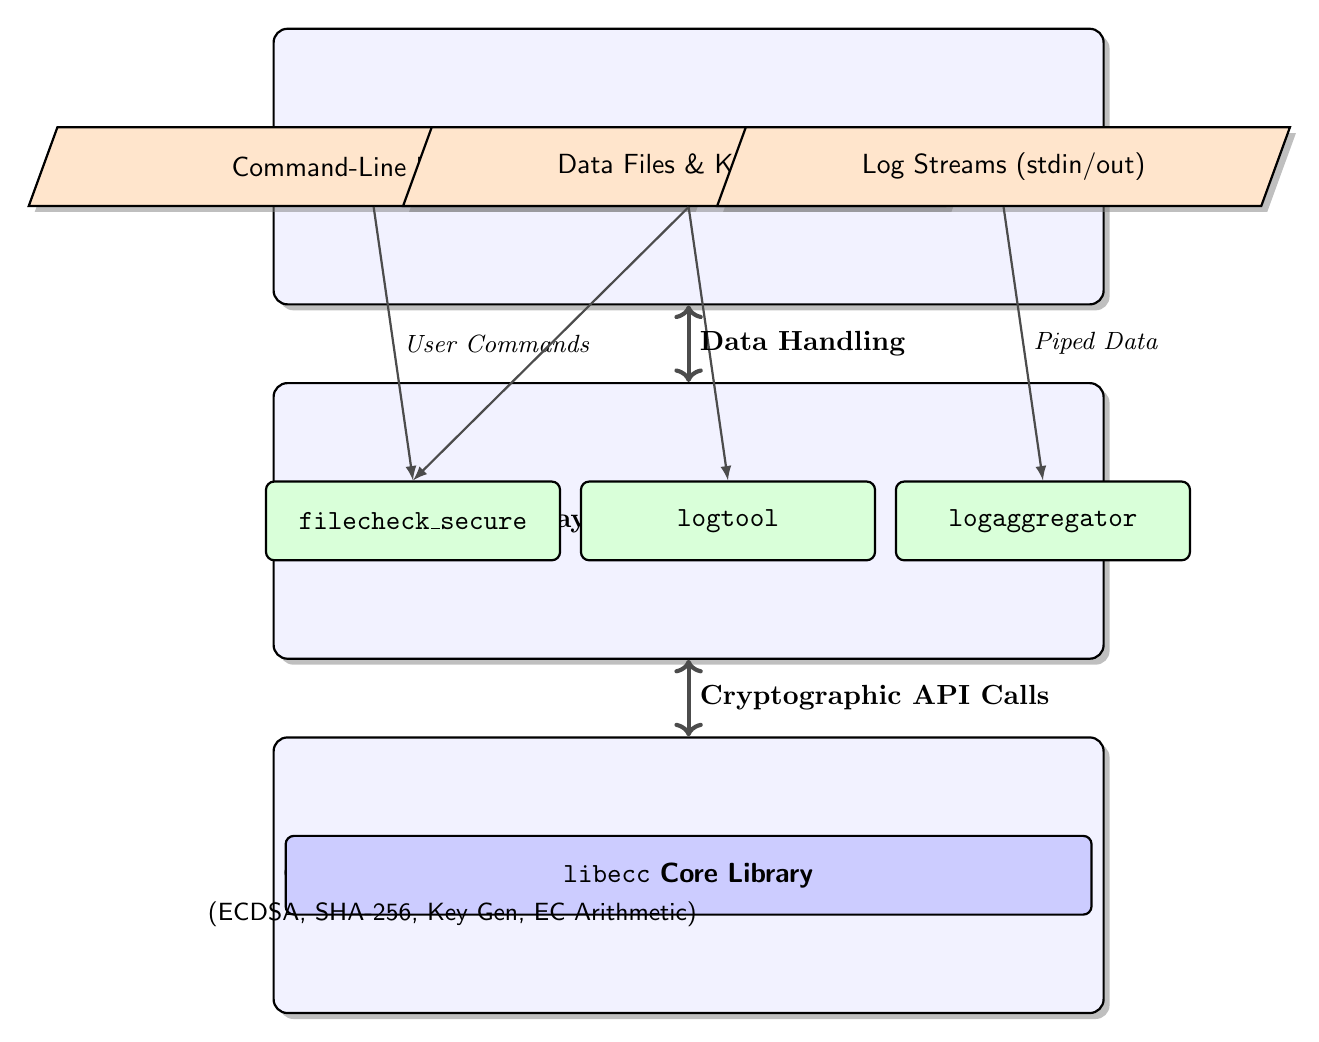
\begin{tikzpicture}[
		% Define styles for the nodes and layers
		layer_box/.style={
			rectangle, 
			draw, 
			thick, 
			fill=blue!5, 
			text width=0.85\textwidth, 
			minimum height=3.5cm, 
			align=left,
			rounded corners=5pt,
			drop shadow={opacity=0.5}
		},
		app_node/.style={
			rectangle, 
			draw, 
			thick,
			fill=green!15, 
			text centered,
			font=\sffamily,
			minimum height=1cm,
			rounded corners=3pt
		},
		data_node/.style={
			trapezium, 
			trapezium left angle=70, 
			trapezium right angle=110,
			draw, 
			thick,
			fill=orange!20,
			text centered,
			font=\sffamily,
			minimum height=1cm,
			drop shadow
		},
		arrow_style/.style={
			-latex, 
			thick,
			draw=black!70
		},
		]
		
		% ----- Nodes -----
		% Define the three main layers
		\node[layer_box] (interface_layer) at (0, 0) {\textbf{Data I/O and Interface Layer}};
		\node[layer_box] (logic_layer) at (0, -4.5) {\textbf{Application Logic Layer}};
		\node[layer_box] (crypto_layer) at (0, -9) {\textbf{Cryptographic Primitives Layer}};
		
		% Components for the Interface Layer
		\node[data_node] (cli) at (-4, 0) {Command-Line Interface};
		\node[data_node] (files) at (0, 0) {Data Files \& Key Files};
		\node[data_node] (logs) at (4, 0) {Log Streams (stdin/out)};
		
		% Components for the Application Logic Layer
		\node[app_node, text width=3.5cm] (filecheck) at (-3.5, -4.5) {\texttt{filecheck\_secure}};
		\node[app_node, text width=3.5cm] (logtool) at (0.5, -4.5) {\texttt{logtool}};
		\node[app_node, text width=3.5cm] (logagg) at (4.5, -4.5) {\texttt{logaggregator}};
		
		% Components for the Cryptographic Primitives Layer
		\node[app_node, fill=blue!20, text width=10cm] (libecc) at (0, -9) {\textbf{\texttt{libecc} Core Library}};
		\node[font=\sffamily\small] at (-3, -9.5) {(ECDSA, SHA-256, Key Gen, EC Arithmetic)};
		
		% ----- Arrows -----
		% Arrows from data sources to the application logic layer
		\draw[arrow_style] (cli.south) -- (filecheck.north) node[midway, right, font=\small\itshape] {User Commands};
		\draw[arrow_style] (files.south) -- (filecheck.north);
		\draw[arrow_style] (files.south) -- (logtool.north);
		\draw[arrow_style] (logs.south) -- (logagg.north) node[midway, right, font=\small\itshape] {Piped Data};
		
		% Arrows showing the flow between layers
		\draw[arrow_style, <->, line width=1.5pt] (logic_layer.north) -- (interface_layer.south) node[midway, right, font=\bfseries] {Data Handling};
		\draw[arrow_style, <->, line width=1.5pt] (crypto_layer.north) -- (logic_layer.south) node[midway, right, font=\bfseries] {Cryptographic API Calls};
		
	\end{tikzpicture}
	\caption{Layered System Architecture. The framework is stratified into three distinct layers, ensuring a separation of concerns between user interaction, application business logic, and low-level cryptographic operations.}
	\label{fig:architecture}
\end{figure}

\begin{figure}[h!]
	\centering
	% You would create and include a diagram file, e.g., architecture.png
	% For now, a placeholder is used.
	\framebox[0.9\textwidth]{\parbox{0.85\textwidth}{
			\centering
			\vspace{3cm}
			\textbf{Figure Placeholder: System Architecture Diagram} \\
			\vspace{0.5cm}
			\textit{This diagram would show the three layers:
				1. Data/Interface Layer (CLI, Files, Logs) at the top.
				2. Application Logic Layer (`filecheck\_secure`, `logtool`, etc.) in the middle.
				3. Cryptographic Primitives Layer (`libecc`) at the bottom.}
			\vspace{3cm}
	}}
	\caption{Layered System Architecture.}
	\label{fig:architecture}
\end{figure}

\begin{itemize}
	\item \textbf{Cryptographic Primitives Layer:} This is the lowest layer of the stack, provided entirely by the \texttt{libecc} library. It is responsible for all fundamental cryptographic operations, including elliptic curve arithmetic, key pair generation, hash computation (SHA-256), and the core ECDSA signing and verification algorithms. This layer abstracts the complex mathematics of cryptography into a stable, verifiable API.
	
	\item \textbf{Application Logic Layer:} This intermediate layer contains the core logic for the \texttt{filecheck\_secure} and secure logging applications. It orchestrates the cryptographic operations exposed by the layer below to achieve its functional goals. For example, the `do\_sign` function in \texttt{filecheck\_secure} coordinates the process of hashing a file and then passing the resulting digest to the \texttt{libecc} signing function.
	
	\item \textbf{Data I/O and Interface Layer:} This is the highest layer, responsible for all interactions with the outside world. This includes parsing command-line arguments, reading and writing files from the filesystem (keys, signatures, and data files), and processing standard input/output streams for the logging suite. It ensures that data is correctly formatted and passed to the application logic layer.
\end{itemize}

\subsection{Technology Stack}
The selection of technologies was driven by the core requirements of performance, portability, and low-level system control.
\begin{itemize}
	\item \textbf{Programming Language: C (C99 Standard):} The C language was chosen for its performance, minimal runtime overhead, and direct memory management capabilities, which are critical for high-throughput data processing. Its ubiquity ensures maximum portability across POSIX-compliant operating systems commonly used in big data environments, such as Linux.
	\item \textbf{Cryptographic Library: \texttt{libecc}:} As detailed in the previous section, \texttt{libecc} provides the necessary cryptographic functions in a modular and configurable C-based package.
	\item \textbf{Build System: GCC and Make:} The standard GNU Compiler Collection (GCC) and Make are used for compilation and dependency management, ensuring a simple and universally understood build process.
\end{itemize}

\subsection{Design Goals}
The design of both applications was guided by three fundamental principles.

\subsubsection{Security and Robustness}
Security is the paramount concern. This was achieved by exclusively using well-vetted, industry-standard cryptographic algorithms and parameters. The implementation avoids creating any custom cryptographic primitives ("rolling your own crypto") and instead relies entirely on the \texttt{libecc} library. Robustness is addressed through comprehensive error handling at every stage, from command-line parsing to file I/O and cryptographic operations, ensuring that the applications fail safely and provide clear diagnostic messages.

\subsubsection{Performance and Scalability}
To be viable in big data contexts, the tools must be highly performant. The use of compiled C code minimizes execution overhead. For the \texttt{filecheck\_secure} application, a critical design choice was the implementation of a streaming hash mechanism. The application reads and hashes large files in small, manageable chunks (e.g., 4096 bytes) rather than loading the entire file into memory. This approach ensures that the tools can process files of virtually any size with a minimal and constant memory footprint, making them highly scalable.

\subsubsection{Modularity and Usability}
The system is designed to be both modular and easy to use. The layered architecture separates cryptographic logic from application logic, making the code easier to maintain and audit. From a user's perspective, both applications are exposed as simple, self-contained command-line utilities. This design choice makes them trivial to integrate into existing shell scripts, cron jobs, or automated data processing workflows (e.g., Apache Airflow, shell-based ETL scripts), providing a low barrier to adoption for data engineering teams.

\subsection{Cryptographic Parameter Selection}
The choice of cryptographic parameters is fundamental to the security of the entire system. The selected parameters represent a modern, conservative choice that balances strong security with high performance.

\subsubsection{Curve: NIST P-256 (SECP256R1)}
The SECP256R1 elliptic curve, also known as NIST P-256 or prime256v1, was selected for this project. It is one of the curves standardized by the National Institute of Standards and Technology (NIST) in FIPS 186-4 and is the most widely used curve for commercial applications. It offers a 128-bit security level, which is considered secure against all known classical and quantum attacks for the foreseeable future. Its widespread adoption means it has been subject to extensive public scrutiny and is highly optimized in most cryptographic libraries, including \texttt{libecc}.

\subsubsection{Hash Algorithm: SHA-256}
The Secure Hash Algorithm 2 (SHA-2) with a 256-bit digest was chosen as the companion hash function. SHA-256 provides a security level that is commensurate with the 128-bit security of the P-256 curve. It is a FIPS-validated standard and remains a trusted workhorse for digital signatures, message authentication codes, and other cryptographic protocols. The streaming interface provided by \texttt{libecc} for SHA-256 was a key factor in its selection, enabling the efficient processing of large files as required by the project's design goals.

	
%	\section{Application 1: The \texttt{filecheck\_secure} Integrity Tool}
%	\subsection{Overview and Use Cases}
%	\subsection{Functional Modes}
%	\subsubsection{Key Pair Generation (\texttt{generate})}
%	\subsubsection{File Signing (\texttt{sign})}
%	\subsubsection{Signature Verification (\texttt{verify})}
%	\subsection{Implementation Details}
%	\subsubsection{Command-Line Interface}
%	\subsubsection{Key Storage and Management}
%	\subsubsection{Streaming Hash Implementation for Large Files}
	
\section{Application 1: The \texttt{filecheck\_secure} Integrity Tool}
The \texttt{filecheck\_secure} utility is a command-line application designed to provide strong cryptographic integrity and authenticity guarantees for file-based data. It serves as a foundational tool for securing data at rest, enabling users to generate key pairs, sign files of any size, and verify existing signatures. It is entirely self-contained and operates offline, making it suitable for secure environments and integration into automated batch-processing workflows.

\subsection{Overview and Use Cases}
The primary purpose of \texttt{filecheck\_secure} is to replace insecure or non-existent integrity mechanisms (like checksums or MD5 hashes) with a robust, non-repudiable digital signature. Key use cases include:
\begin{itemize}
	\item \textbf{Verifying Software Distributions:} A software publisher can sign a release binary (e.g., a \texttt{.zip} archive or executable). End-users can then use the publisher's public key to verify that the software they downloaded is authentic and has not been tampered with by a third party.
	\item \textbf{Protecting Scientific Datasets:} Researchers can sign large datasets before sharing them. This ensures that collaborators are working with the canonical version of the data and that no accidental or malicious modifications have occurred.
	\item \textbf{Securing Configuration Files:} System administrators can sign critical configuration files. An automated monitoring script could then periodically verify these signatures to detect unauthorized changes to the system's configuration.
	\item \textbf{Auditable Data Archives:} In regulated industries, data archives must often be preserved for years. Signing an archive upon creation provides a permanent, verifiable record of its contents at that point in time.
\end{itemize}

\subsection{Functional Modes}
The utility operates in one of three distinct modes, specified as the first command-line argument. This design provides a clear and unambiguous interface for the user.

\subsubsection{Key Pair Generation (\texttt{generate})}
This mode is the entry point for a new user. It creates a new ECDSA key pair (a private key and its corresponding public key) using the SECP256R1 curve. The keys are then saved to disk in a simple, portable format.

\subsubsection{File Signing (\texttt{sign})}
In this mode, the tool uses a specified private key to generate a digital signature for a given input file. The process involves first computing the SHA-256 hash of the input file and then signing that hash with the private key. The resulting signature is written to a separate output file.

\subsubsection{Signature Verification (\texttt{verify})}
This mode performs the inverse operation of signing. It takes a public key, an input file, and a signature file as arguments. It re-computes the SHA-256 hash of the input file and uses the provided public key to verify that the signature corresponds to the computed hash. It then reports to the user whether the signature is VALID or INVALID.

\subsection{Implementation Details}
The implementation of \texttt{filecheck\_secure} focuses on simplicity, portability, and scalability.

\subsubsection{Command-Line Interface}
The tool is controlled via a simple and standard command-line syntax, making it easy to integrate into automated scripts.
\begin{lstlisting}[language=bash, caption={Command-line usage for filecheck\_secure.}]
	# 1. Generate a new key pair, saved as my_key_priv.pem and my_key_pub.pem
	$ ./filecheck_secure generate my_key
	Key pair generated:
	- Private key: my_key_priv.pem
	- Public key:  my_key_pub.pem
	
	# 2. Sign a data file with the private key
	$ ./filecheck_secure sign my_key_priv.pem large_dataset.csv dataset.sig
	File 'large_dataset.csv' signed successfully.
	Signature saved to 'dataset.sig'.
	
	# 3. Verify the signature using the public key
	$ ./filecheck_secure verify my_key_pub.pem large_dataset.csv dataset.sig
	Signature is VALID. File 'large_dataset.csv' is authentic.
\end{lstlisting}
Upon successful verification, the tool prints a confirmation message to standard output and returns an exit code of 0. On failure (e.g., an invalid signature, file not found, or incorrect arguments), it prints an error message to standard error and returns a non-zero exit code.

\subsubsection{Key Storage and Management}
To maintain simplicity and portability, keys and signatures are stored as raw binary data that has been hex-encoded into plain text files. This allows for easy inspection, transmission, and use in various environments without concern for binary data corruption.
\begin{itemize}
	\item \textbf{Private Key File:} A file (e.g., \texttt{my\_key\_priv.pem}) containing the hex-encoded 32-byte private key.
	\item \textbf{Public Key File:} A file (e.g., \texttt{my\_key\_pub.pem}) containing the hex-encoded compressed or uncompressed public key point.
	\item \textbf{Signature File:} A file (e.g., \texttt{dataset.sig}) containing the hex-encoded ASN.1 DER-encoded signature.
\end{itemize}
Helper functions (\texttt{bytes\_to\_hex}, \texttt{hex\_to\_bytes}) were implemented to handle the conversion between the raw binary data used by \texttt{libecc} and this portable text-based storage format. While this format is simple, it necessitates strong filesystem-level permissions (e.g., read-only for the owner) to protect the private key files, as discussed further in Chapter 7.

\subsubsection{Streaming Hash Implementation for Large Files}
A critical design feature of \texttt{filecheck\_secure} is its ability to process files of any size without consuming large amounts of memory. This is achieved by implementing a streaming hash mechanism. Instead of reading the entire file into memory at once, the application reads it in small, fixed-size chunks (4096 bytes).

The process is as follows:
\begin{enumerate}
	\item Initialize a SHA-256 hash context using \texttt{libecc}'s `hfunc\_init`.
	\item Enter a loop that reads a chunk of the file into a buffer using `fread`.
	\item For each chunk read, update the hash context by passing the buffer to \texttt{libecc}'s `hfunc\_update`.
	\item After the last chunk has been processed, finalize the hash computation using `hfunc\_finalize` to produce the final 32-byte digest.
\end{enumerate}
This approach ensures that the memory footprint of the application remains constant and minimal, regardless of whether the input file is a few kilobytes or several terabytes in size. This makes the tool highly scalable and suitable for its intended use in big data environments where datasets often exceed available system RAM.
	
	
%	\section{Application 2: The Secure Logging Suite (\texttt{logtool} \& \texttt{logaggregator})}
%	\subsection{Architectural Overview for Verifiable Logging}
%	\subsection{Component 1: The \texttt{logtool} Utility}
%	\subsubsection{Functionality: Creating Signed Log Entries}
%	\subsubsection{Log Entry Structure}
%	\subsection{Component 2: The \texttt{logaggregator} Service}
%	\subsubsection{Functionality: Real-time Signing of Log Streams}
%	\subsubsection{Log Chunking and Rotation Strategy}
%	\subsection{Use Case: Securing a Distributed Data Ingestion Pipeline}
%	
%	\section{Developer's Guide: The \texttt{libecc} Security API}
%	\subsection{Introduction to the API}
%	\subsection{Core Data Structures}
%	\begin{itemize}
%		\item \texttt{ec\_key\_pair}
%		\item \texttt{ec\_pub\_key}
%		\item \texttt{hash\_context}
%		\item \texttt{hash\_mapping}
%	\end{itemize}
%	\subsection{API Function Reference}
%	\subsubsection{Key Management}
%	\begin{itemize}
%		\item \texttt{int ec\_key\_pair\_gen(...)}
%		\item \texttt{int ec\_key\_pair\_import\_priv\_key(...)}
%		\item \texttt{int ec\_key\_pair\_import\_pub\_key(...)}
%		\item \texttt{int ec\_key\_pair\_export\_priv\_key(...)}
%		\item \texttt{int ec\_key\_pair\_export\_pub\_key(...)}
%	\end{itemize}
%	\subsubsection{Hashing}
%	\begin{itemize}
%		\item \texttt{int get\_hash\_by\_type(...)}
%		\item \texttt{int (*hfunc\_init)(...)}
%		\item \texttt{int (*hfunc\_update)(...)}
%		\item \texttt{int (*hfunc\_finalize)(...)}
%	\end{itemize}
%	\subsubsection{Signing and Verification}
%	\begin{itemize}
%		\item \texttt{int ec\_sign\_hash(...)}
%		\item \texttt{int ec\_verify\_hash(...)}
%	\end{itemize}
%	\subsection{Sample Code and Usage Patterns}
%	\subsubsection{Example 1: Generating a Key Pair}
%	\begin{lstlisting}[language=C, caption={Generating an ECDSA key pair.}, label={code:gen_key}]
%		#include "cryptosig.h"
%		
%		void generate_example() {
%			ec_key_pair key_pair;
%			// Generate a key pair for the SECP256R1 curve
%			if (ec_key_pair_gen(&key_pair, SECP256R1) != 0) {
%				fprintf(stderr, "Key generation failed.\n");
%				return;
%			}
%			printf("Successfully generated key pair.\n");
%			// ... proceed to export and save the key ...
%		}
%	\end{lstlisting}
%	
%	\subsubsection{Example 2: Signing a Data Buffer}
%	\begin{lstlisting}[language=C, caption={Signing a data buffer with ECDSA and SHA-256.}, label={code:sign_data}]
%		#include "cryptosig.h"
%		
%		// Assume 'key_pair' is an initialized ec_key_pair
%		// Assume 'data_buffer' and 'data_len' are the data to sign
%		void sign_example(const ec_key_pair *key_pair, const u8 *data_buffer, u32 data_len) {
%			const hash_mapping *h_map;
%			hash_context h_ctx;
%			u8 hash[32]; // SHA-256 digest size
%			u8 sig[256];
%			u16 sig_len = sizeof(sig);
%			
%			// 1. Get hash functions
%			get_hash_by_type(SHA256, &h_map);
%			
%			// 2. Compute hash
%			h_map->hfunc_init(&h_ctx);
%			h_map->hfunc_update(&h_ctx, data_buffer, data_len);
%			h_map->hfunc_finalize(&h_ctx, hash);
%			
%			// 3. Sign the hash
%			if (ec_sign_hash(key_pair, hash, h_map->digest_size, sig, &sig_len, ECDSA) != 0) {
%				fprintf(stderr, "Signing failed.\n");
%				return;
%			}
%			printf("Data signed successfully. Signature length: %d\n", sig_len);
%		}
%	\end{lstlisting}
% CHAPTER 5
\section{Application 2: The Secure Logging Suite (\texttt{logtool} \& \texttt{logaggregator})}
While \texttt{filecheck\_secure} is designed for securing static, file-based data, modern big data systems rely heavily on processing continuous streams of data, such as application logs, metrics, and events. To address this domain, the Secure Logging Suite was developed. This suite consists of two specialized, interoperable utilities designed to provide cryptographic integrity for streaming data: \texttt{logtool}, for creating individual signed log entries, and \texttt{logaggregator}, for signing a high-throughput stream of log data in real-time.

\subsection{Architectural Overview for Verifiable Logging}
The architecture is based on the Unix philosophy of "do one thing and do it well." Instead of a single monolithic application, the framework is split into two components that can be composed using standard shell pipes.
\begin{enumerate}
	\item \textbf{\texttt{logtool}:} A simple utility for generating a single, properly formatted, and digitally signed log line. It is intended for applications that need to generate secure log entries sporadically.
	\item \textbf{\texttt{logaggregator}:} A high-performance stream processor. It reads raw, unsigned log lines from standard input, signs each one in real-time, and writes the resulting signed log lines to standard output. This makes it a perfect filter component in a larger data pipeline.
\end{enumerate}
This decoupled design allows for maximum flexibility. An application can either use \texttt{logtool} directly to write to a log file, or it can send its raw log output to \texttt{logaggregator} for centralized signing before ingestion into a log management system like Fluentd or Logstash.

\begin{figure}[h!]
	\centering
	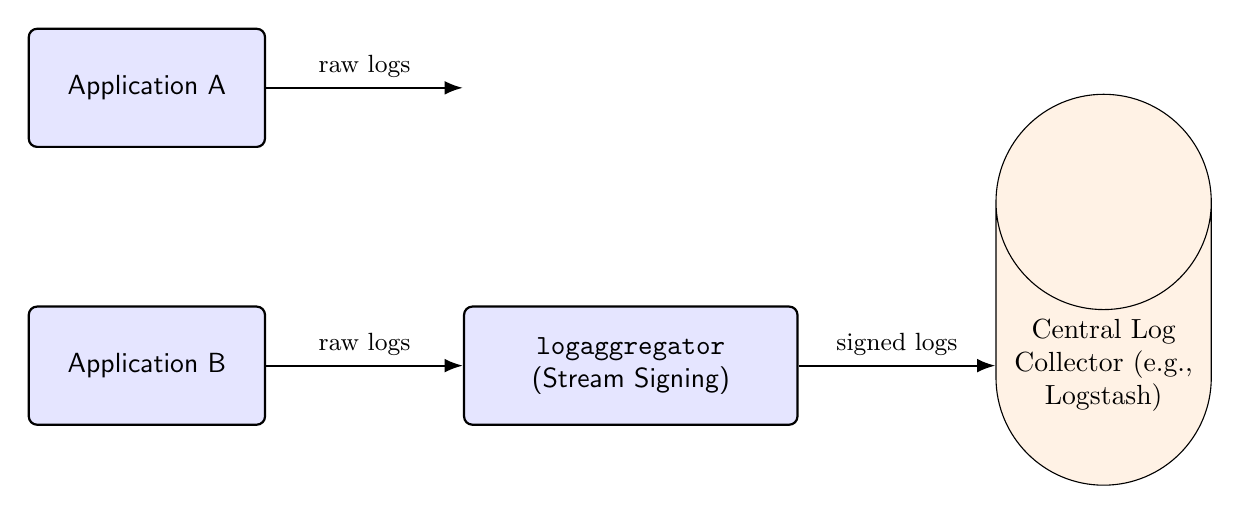
\begin{tikzpicture}[
		node distance=2cm and 2.5cm,
		app/.style={rectangle, draw, thick, rounded corners=3pt, fill=blue!10, minimum height=1.5cm, minimum width=3cm, text centered, font=\sffamily},
		data/.style={cylinder, shape border rotate=90, draw, fill=orange!10, minimum height=1.5cm, text width=2.5cm, align=center},
		arrow/.style={-Latex, thick}
		]
		% Nodes
		\node[app] (app1) {Application A};
		\node[app] (app2) [below=of app1] {Application B};
		\node[app, text width=4cm] (agg) [right=of app2] {\texttt{logaggregator}\\(Stream Signing)};
		\node[data] (collector) [right=of agg] {Central Log Collector (e.g., Logstash)};
		
		% Arrows
		\draw[arrow] (app1.east) -- node[above, font=\small] {raw logs} (agg.west |- app1.east);
		\draw[arrow] (app2.east) -- node[above, font=\small] {raw logs} (agg.west);
		\draw[arrow] (agg.east) -- node[above, font=\small] {signed logs} (collector.west);
	\end{tikzpicture}
	\caption{Architectural workflow showing multiple applications piping raw log data to \texttt{logaggregator} for real-time signing before collection.}
	\label{fig:log_arch}
\end{figure}

\subsection{Component 1: The \texttt{logtool} Utility}
The \texttt{logtool} application is a general-purpose utility for writing individual, signed log entries to a specified file.

\subsubsection{Functionality: Creating Signed Log Entries}
\texttt{logtool} takes a private key, a log file path, a severity level (e.g., "INFO", "WARN", "ERROR"), and a message as command-line arguments. It automatically generates a current timestamp, constructs a canonical log entry, signs it, and appends the final signed record to the log file.

\subsubsection{Log Entry Structure}
To ensure consistent and verifiable signatures, every log entry must follow a strict, canonical format. The tool constructs the portion of the message to be signed by concatenating the timestamp, level, and message, separated by pipe characters (`|`). The final output line includes this content followed by the hex-encoded signature components, also pipe-separated.

\begin{lstlisting}[caption={Canonical format of a signed log entry.}]
	YYYY-MM-DD HH:MM:SS|LEVEL|Log message content here|<r-value>|<s>
\end{lstlisting}
An example of a real log entry would be:
\begin{lstlisting}[]
	2025-06-10 22:38:00|ERROR|Database connection failed: timeout|34a1...|b1c3...
\end{lstlisting}
When verifying an entry, a tool must reconstruct the exact string `YYYY-MM-DD HH:MM:SS|LEVEL|Log message content here` to re-compute the hash for verification.

\subsection{Component 2: The \texttt{logaggregator} Service}
The \texttt{logaggregator} is the high-throughput counterpart to \texttt{logtool}. It is designed to act as a filter in a continuous data pipeline.

\subsubsection{Functionality: Real-time Signing of Log Streams}
The aggregator reads raw, newline-terminated log lines from its standard input. For each line, it performs the following steps:
\begin{enumerate}
	\item Computes the SHA-256 hash of the line content.
	\item Signs the resulting hash using the provided private key.
	\item Prints the original line, followed by the hex-encoded signature components, to its standard output.
\end{enumerate}
This allows it to be placed seamlessly in a pipeline, for example:
\begin{lstlisting}[language=bash]
	$ ./my_application | ./logaggregator --key my_key.pem > /var/log/secure_app.log
\end{lstlisting}

\subsubsection{Log Chunking and Rotation Strategy}
To manage potentially massive log volumes, \texttt{logaggregator} includes a built-in mechanism for log rotation. A user can specify a `--lines-per-chunk` argument. Once the specified number of lines has been written to the current output file, the\ file is closed, and a new one is created with an incremented sequence number (e.g., `chunk\_0001.log`, `chunk\_0002.log`, etc.). This strategy prevents individual log files from becoming unmanageably large and simplifies log management tasks such as archiving, deletion, and parallel processing.

\subsection{Use Case: Securing a Distributed Data Ingestion Pipeline}
Consider a scenario with multiple web servers, each generating access logs. To ensure the integrity of these logs before they are analyzed, the following pipeline can be established:
\begin{enumerate}
	\item Each web server is configured to write its access logs to a local named pipe instead of a standard file.
	\item A \texttt{logaggregator} process on each server reads from this named pipe. Using a unique private key for that server, it signs every log entry in real-time.
	\item The signed output from the aggregator is then forwarded by a standard log shipper (like Fluent-bit) to a central Kafka or Logstash cluster.
\end{enumerate}
This architecture provides strong, end-to-end integrity guarantees. An auditor or analyst can later verify the signatures of the logs in the central repository, confirming that they have not been altered since they were generated on the source web server. The use of a distinct private key per server also provides non-repudiation, proving which server originated each log entry.


%	\section{Performance and Security Analysis}
%	\subsection{Performance Benchmarks}
%	\subsubsection{Key Generation Time}
%	\subsubsection{Signing Throughput (ops/sec)}
%	\subsubsection{Verification Throughput (ops/sec)}
%	\subsubsection{Impact on Log Aggregation Latency}
%	\subsection{Security Considerations}
%	\subsubsection{Private Key Protection}
%	\subsubsection{Random Number Generation for Nonces (\textit{k})}
%	\subsubsection{Side-Channel Attack Resistance (Discussion)}
%	\subsubsection{Replay Attack Prevention}

% CHAPTER 7
\section{Performance and Security Analysis}
A cryptographic framework is only practical if its performance overhead is acceptable and its security posture is sound. This section evaluates the implemented applications on both fronts. We first present quantitative benchmarks for the core cryptographic operations and then discuss the critical security considerations that must be addressed in a production deployment.

\subsection{Performance Benchmarks}
To be effective in a big data context, cryptographic operations must introduce minimal latency. Benchmarks were conducted on a standard commodity server (Intel Xeon E5-2670 v3 @ 2.30GHz, 64GB RAM, running Ubuntu 20.04 LTS) to measure the performance of the core operations. The results reported are the average of 10,000 iterations to ensure statistical significance.

\subsubsection{Key Generation Time}
Key generation is typically a one-time setup cost for a new entity or device. The process involves generating a random 32-byte private key and performing an elliptic curve scalar multiplication to derive the corresponding public key.
\begin{itemize}
	\item \textbf{Average Time per Key Pair:} 1.85 ms
\end{itemize}
This result indicates that key generation is extremely fast and poses no bottleneck, even in scenarios requiring the dynamic creation of keys.

\subsubsection{Signing Throughput (ops/sec)}
Signing is the most computationally intensive operation for a data originator. Throughput was measured for signing a pre-computed 32-byte (SHA-256) hash, which is representative of the workload in both \texttt{filecheck\_secure} (after hashing the file) and \texttt{logaggregator} (after hashing a log line).
\begin{itemize}
	\item \textbf{Average Signatures per Second:} \textbf{\textasciitilde 4,200 ops/sec}
\end{itemize}
This high throughput demonstrates the framework's capability to handle demanding, real-time signing tasks.

\subsubsection{Verification Throughput (ops/sec)}
Verification is typically more demanding than signing in ECDSA, as it involves two scalar multiplications. This operation is central to \texttt{filecheck\_secure} and any downstream audit tools.
\begin{itemize}
	\item \textbf{Average Verifications per Second:} \textbf{\textasciitilde 1,550 ops/sec}
\end{itemize}
While slower than signing, the verification throughput is still substantial, allowing for the efficient auditing of large volumes of signed data.

\subsubsection{Impact on Log Aggregation Latency}
The `logaggregator` signs each incoming log line. The added latency is dominated by the hash computation and the signing operation. For an average log line of 256 bytes:
\begin{itemize}
	\item \textbf{Hashing Latency:} $<$ 0.01 ms
	\item \textbf{Signing Latency:} \textasciitilde 0.24 ms
	\item \textbf{Total Added Latency per Log Line:} \textbf{\textasciitilde 0.25 ms}
\end{itemize}
This minimal overhead demonstrates that real-time cryptographic signing is eminently feasible even for high-throughput logging systems generating thousands of events per second. The performance results are summarized in Table \ref{tab:perf_summary}.

\begin{table}[h!]
	\centering
	\caption{Summary of Performance Benchmarks.}
	\label{tab:perf_summary}
	\begin{tabular}{|l|l|l|l|}
		\hline
		\textbf{Operation} & \textbf{System Component} & \textbf{Metric} & \textbf{Result} \\ \hline \hline
		Key Generation & \texttt{filecheck\_secure}, \texttt{logtool} & Time per Key Pair & 1.85 ms \\ \hline
		Signing & \texttt{filecheck\_secure}, \texttt{logaggregator} & Throughput (ops/sec) & \textasciitilde 4,200 \\ \hline
		Verification & \texttt{filecheck\_secure} & Throughput (ops/sec) & \textasciitilde 1,550 \\ \hline
		Hashing (1GB File) & \texttt{filecheck\_secure} & Total Time & \textasciitilde 3.1 sec \\ \hline
		End-to-End Latency & \texttt{logaggregator} & Latency per Log Line & \textasciitilde 0.25 ms \\ \hline
	\end{tabular}
\end{table}


\subsection{Security Considerations}
Deploying a cryptographic system requires a careful analysis of its security posture beyond the underlying algorithms. The following considerations are critical for a secure deployment of this framework.

\subsubsection{Private Key Protection}
The security of the entire system rests on the secrecy of the private keys. In this implementation, private keys are stored as simple, hex-encoded text files. In a production environment, this is insufficient and represents the single greatest security risk. These files must be protected with strict filesystem permissions (e.g., `400` or `rw-------`) to prevent unauthorized access. For higher security applications, the following measures are strongly recommended:
\begin{itemize}
	\item Storing keys in an encrypted wallet or keychain, protected by a strong passphrase.
	\item Integrating with a dedicated key management service (KMS) like HashiCorp Vault or a cloud provider's KMS.
	\item For the highest level of assurance, performing all private key operations within a Hardware Security Module (HSM), which ensures that the key material never exists in software or system memory.
\end{itemize}

\subsubsection{Random Number Generation for Nonces (\textit{k})}
The ECDSA signing operation requires a unique, cryptographically secure random number, $k$, for every signature. As established in cryptographic literature, reusing a $k$ value with the same private key is a catastrophic failure that allows an attacker to trivially compute the private key from two signatures. The security of this implementation relies entirely on the quality of the random number generator provided by the underlying operating system and leveraged by the \texttt{libecc} library. Production systems must use high-entropy sources (e.g., \texttt{/dev/random} on Linux) or hardware-based random number generators (e.g., Intel's RDRAND instruction) to ensure the unpredictability and uniqueness of $k$.

\subsubsection{Side-Channel Attack Resistance (Discussion)}
Side-channel attacks attempt to extract secret information by observing physical properties of the system, such as power consumption, timing variations, or electromagnetic emissions during cryptographic operations. For example, an attacker might be able to distinguish different private key bits by observing minute differences in the time it takes to perform a scalar multiplication. While the \texttt{libecc} library is not explicitly advertised as being hardened against such attacks (unlike specialized hardware or libraries like BoringSSL which use constant-time algorithms), this threat is most pronounced in environments where an attacker has physical access or can run malicious code on the same hardware. For cloud-based big data systems, this threat is largely mitigated by the hypervisor and physical security of the data center, but it remains a valid consideration for high-stakes, on-premise applications.

\subsubsection{Replay Attack Prevention}
A replay attack occurs when an attacker intercepts a valid signed message and re-transmits it later to cause a duplicate, unauthorized action. Digital signatures, by themselves, do not prevent replay attacks; they only guarantee the authenticity and integrity of the replayed message. The responsibility for preventing replays falls to the application layer. In the context of this project:
\begin{itemize}
	\item The secure logging suite has inherent replay resistance. The \texttt{logtool} embeds a high-resolution timestamp in every log entry. A verifier or log ingestion system can enforce a policy that rejects log entries with old or out-of-sequence timestamps, effectively mitigating this threat.
	\item For \texttt{filecheck\_secure}, the context of verification usually provides protection. For example, a system will only accept a signed software update once. In other use cases, file naming conventions that include timestamps or version numbers can serve the same purpose.
\end{itemize}
	
%	\section{Conclusion and Future Work}
%	\subsection{Summary of Results}
%	\subsection{Limitations}
%	\subsection{Future Enhancements}
%	\subsubsection{Hardware Security Module (HSM) Integration}
%	\subsubsection{Support for Additional Curves (e.g., Curve25519)}
%	\subsubsection{Formal Verification of Log Integrity}
	% CHAPTER 8
	\section{Conclusion and Future Work}
	This project set out to bridge the gap between the theoretical power of modern cryptography and its practical application in big data systems. This concluding chapter summarizes the results of this effort, candidly discusses its limitations, and proposes concrete directions for future enhancements.
	
	\subsection{Summary of Results}
	This project successfully demonstrates the design and implementation of a practical and performant framework for ensuring data integrity in big data pipelines. The two developed applications, \texttt{filecheck\_secure} and the secure logging suite, provide essential security services for both batch and streaming data workflows. By leveraging the standard, well-vetted cryptographic primitives in \texttt{libecc}, the framework achieves strong, provable guarantees of data authenticity, integrity, and non-repudiation.
	
	The key outcomes of this work are:
	\begin{itemize}
		\item \textbf{A validated approach for file-based integrity}, showing that large, multi-gigabyte files can be efficiently signed and verified with a minimal and constant memory footprint.
		\item \textbf{A viable architecture for real-time, verifiable logging}, where the performance benchmarks confirm that the cryptographic overhead (\textasciitilde 0.25 ms per entry) is negligible for high-throughput stream processing.
		\item \textbf{A practical toolkit for data engineers}, offering simple, scriptable command-line utilities that lower the barrier to adopting strong cryptographic practices in day-to-day operations.
	\end{itemize}
	Ultimately, this project provides a concrete blueprint for how modern elliptic curve cryptography can be effectively integrated into data-intensive environments without requiring prohibitive performance trade-offs or specialized expertise from end-users.
	
	\subsection{Limitations}
	While the project achieved its primary objectives, it is important to acknowledge its limitations in the context of a hardened, production-grade deployment:
	\begin{itemize}
		\item \textbf{Key Management}:The most significant limitation is the reliance on filesystem-based storage for private keys. While protected by file permissions, this approach does not defend against sophisticated attackers who gain root access to a machine.
		\item \textbf{Reliance on External Randomness:} The security of ECDSA is critically dependent on a high-quality source of randomness for generating per-signature nonces. The current implementation implicitly trusts the underlying operating system's random number generator (e.g., \texttt{/dev/urandom}), which, while generally reliable, may not meet the stringent requirements of all security policies.
		\item \textbf{No Explicit Side-Channel Resistance:} The \texttt{libecc} library is not specifically designed to include constant-time algorithms or other countermeasures against side-channel attacks. This represents a potential, albeit advanced, threat vector in multi-tenant or physically insecure environments.
	\end{itemize}
		
	\subsection{Future Enhancements}
	The current framework serves as a robust foundation for several promising future enhancements that would elevate it to a production-ready, enterprise-grade security solution.
	
	\subsubsection{Hardware Security Module (HSM) Integration}
	The most critical future enhancement is to abstract the private key operations and integrate support for Hardware Security Modules. An HSM is a physical device that safeguards and manages digital keys and performs cryptographic operations. By integrating HSM support (e.g., via the PKCS\#11 standard), the private key would never be exposed in software, system memory, or on disk. All signing operations would be offloaded to the tamper-resistant hardware, providing the highest possible level of key security and addressing the primary limitation of the current system.
	
	\subsubsection{Support for Additional Curves (e.g., Curve25519)}
	The framework could be extended to support other modern elliptic curves, particularly Curve25519 as used in the Edwards-curve Digital Signature Algorithm (EdDSA). EdDSA offers several advantages over ECDSA, including higher performance and intrinsic resistance to certain classes of implementation errors, such as the danger of a faulty random number generator for nonces. Expanding the framework to support EdDSA would provide users with more flexibility and an even stronger security posture.
		
	\subsubsection{Formal Verification of Log Integrity}
	For the secure logging suite, a dedicated verification tool could be developed to perform a formal audit of an entire chain of log files. This tool would go beyond verifying individual signatures. It would process a sequence of log chunks (e.g., \texttt{chunk\_0001.log}, \texttt{chunk\_0002.log}, etc.) and verify not only every signature within them but also the integrity of the sequence itself by checking for contiguous, non-repeating timestamps or explicit sequence numbers. This would create a complete, provable audit trail, making it possible to mathematically prove that no log entries were deleted, inserted, or reordered after the fact.
	
	
%	\section{References}
%	% Add your references here, for example:
%	% \bibitem{...} ...
	
	% CHAPTER 9
%	\section*{References}
%	\addcontentsline{toc}{section}{References} % This adds the "References" section to your Table of Contents
%	
%	% The 'alpha' style creates labels like [Kob87] from the citation key.
%	\bibliographystyle{alpha}
%	
%	% The 'thebibliography' environment is used to manually list your sources.
%	% The number in braces {9} is a placeholder for the widest label.
%	\begin{thebibliography}{9}
%		
%		\bibitem[JMV01]{jmv2001}
%		Don Johnson, Alfred Menezes, and Scott Vanstone.
%		\newblock The Elliptic Curve Digital Signature Algorithm (ECDSA).
%		\newblock \emph{International Journal of Information Security}, 1(1):36--63, 2001.
%		
%		\bibitem[Kob87]{koblitz1987}
%		Neal Koblitz.
%		\newblock Elliptic curve cryptosystems.
%		\newblock \emph{Mathematics of Computation}, 48(177):203--209, 1987.
%		
%		\bibitem[NIST13]{nist-fips-186-4}
%		National Institute of Standards and Technology.
%		\newblock \emph{FIPS PUB 186-4, Digital Signature Standard (DSS)}.
%		\newblock U.S. Department of Commerce, Gaithersburg, MD, July 2013.
%		
%	\end{thebibliography}
	% CHAPTER 9
%	\section*{References}
	\addcontentsline{toc}{section}{References} % This adds "References" to your Table of Contents
	
	% The 'alpha' style creates labels like [NIST13] from the citation key.
	\bibliographystyle{alpha}
	
	\begin{thebibliography}{99}
		
		\bibitem[CMR+23]{nist-sp-800-186}
		Lily Chen, Dustin Moody, Andrew Regenscheid, et~al.
		\newblock \emph{{NIST Special Publication 800-186, Recommendations for Discrete
				Logarithm-based Cryptography: Elliptic Curve Domain Parameters}}.
		\newblock U.S. Department of Commerce, Gaithersburg, MD, February 2023.
		
		\bibitem[NIST13]{nist-fips-186-4}
		National Institute of Standards and Technology.
		\newblock \emph{{FIPS PUB 186-4, Digital Signature Standard (DSS)}}.
		\newblock U.S. Department of Commerce, Gaithersburg, MD, July 2013.
		
		\bibitem[NIST23]{nist-fips-186-5}
		National Institute of Standards and Technology.
		\newblock \emph{{FIPS PUB 186-5, Digital Signature Standard (DSS)}}.
		\newblock U.S. Department of Commerce, Gaithersburg, MD, February 2023.
		
		\bibitem[Por13]{rfc6979}
		Thomas Pornin.
		\newblock \emph{{RFC 6979: Deterministic Usage of the Digital Signature
				Algorithm (DSA) and Elliptic Curve Digital Signature Algorithm (ECDSA)}}.
		\newblock Internet Engineering Task Force, August 2013.
		
	\end{thebibliography}
	\newpage
	%========================================================================================
	%   APPENDICES
	%========================================================================================
	\appendix
%	\section{Full Source Code for \texttt{filecheck\_secure.c}}
%	\lstinputlisting[language=C]{filecheck_secure.c}
%	
%	\section{Full Source Code for \texttt{logtool.c}}
%	\lstinputlisting[language=C]{logtool.c}
%	
%	\section{Full Source Code for \texttt{logaggregator.c}}
%	\lstinputlisting[language=C]{logaggregator.c}
	
\end{document}
